\documentclass[tikz,border=8pt]{standalone}
% Shared look for every TikZ diagram. Load with \input{../../tools/tikz-style.tex}
\usepackage[T1]{fontenc}
\usepackage{lmodern}
\renewcommand{\sfdefault}{lmr}  % diagrams use the same serif as the text
\usetikzlibrary{arrows.meta, positioning, shapes.geometric, calc, fit, backgrounds}
\definecolor{cblue}{HTML}{4C78A8}
\definecolor{corange}{HTML}{F58518}
\definecolor{cgreen}{HTML}{54A24B}
\definecolor{cred}{HTML}{E45756}
\definecolor{cpurple}{HTML}{B279A2}
\definecolor{cgrey}{HTML}{6B6B6B}
\tikzset{
  every picture/.style={font=\sffamily, line width=1.2pt},
  box/.style={draw=#1, fill=#1!12, rounded corners=4pt, align=center, inner sep=7pt, minimum height=1.1cm},
  box/.default=cgrey,
  arrow/.style={-{Stealth[length=3mm]}, draw=cgrey, line width=1.4pt},
  title/.style={font=\sffamily\bfseries\Large},
  note/.style={font=\sffamily\small, text=cgrey, align=center},
}
\AtBeginDocument{\hyphenpenalty=10000 \exhyphenpenalty=10000}

\begin{document}
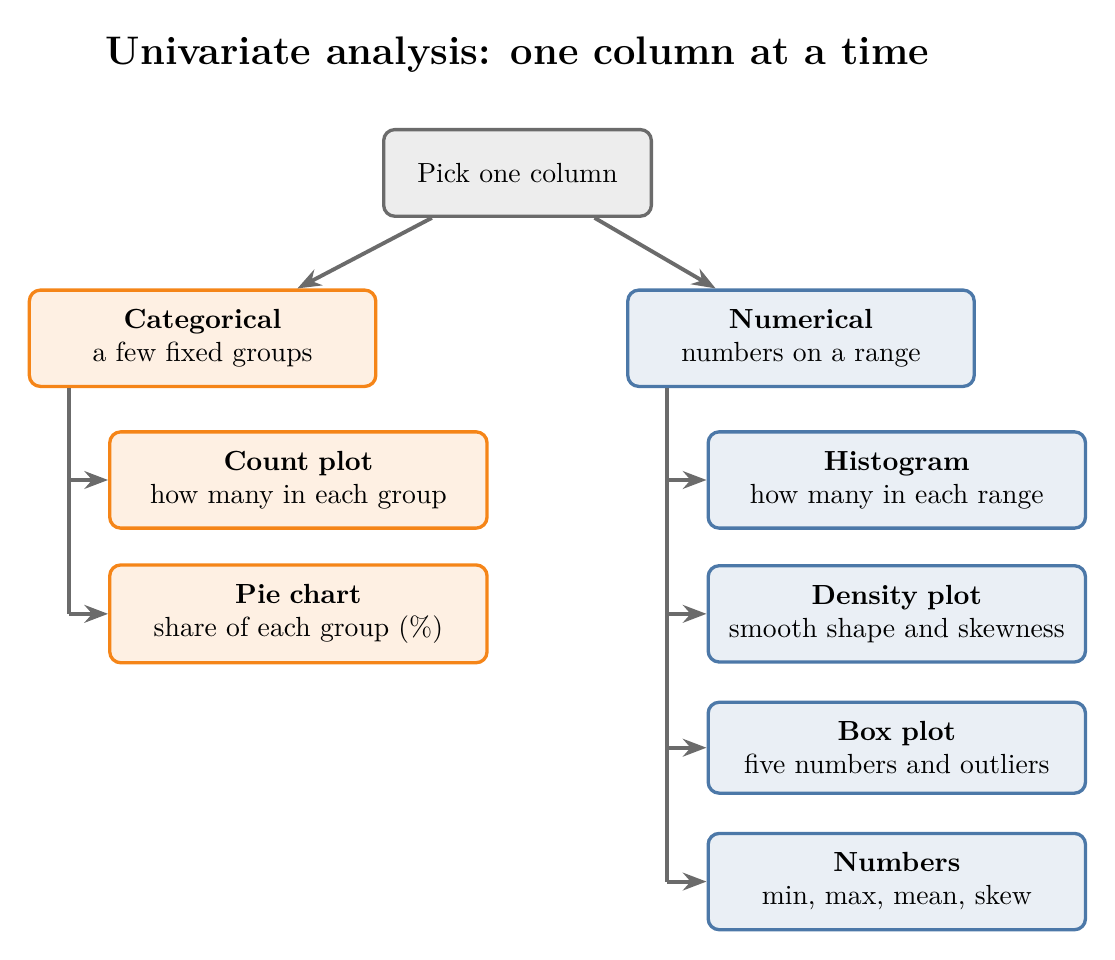
\begin{tikzpicture}
  \node[title] at (5.2,1.5) {Univariate analysis: one column at a time};
  \node[box=cgrey, minimum width=3.4cm] (col) at (5.2,0) {Pick one column};
  \node[box=corange, minimum width=4.4cm] (cat) at (1.2,-2.1) {\textbf{Categorical}\\ a few fixed groups};
  \node[box=cblue, minimum width=4.4cm] (num) at (8.8,-2.1) {\textbf{Numerical}\\ numbers on a range};
  \draw[arrow] (col) -- (cat);
  \draw[arrow] (col) -- (num);
  % plot boxes hang off a vertical spine under each type
  \tikzset{child/.style={box=#1, text width=4.3cm, anchor=west}}
  \foreach \n/\t/\s/\y in {count/Count plot/how many in each group/-3.9, pie/Pie chart/share of each group (\%)/-5.6}
    \node[child=corange] (\n) at (0.0,\y) {\textbf{\t}\\ \s};
  \foreach \n/\t/\s/\y in {hist/Histogram/how many in each range/-3.9, kde/Density plot/smooth shape and skewness/-5.6,
                           bx/Box plot/five numbers and outliers/-7.3, nums/Numbers/{min, max, mean, skew}/-9.0}
    \node[child=cblue] (\n) at (7.6,\y) {\textbf{\t}\\ \s};
  \draw[cgrey, line width=1.4pt] (-0.5,-2.1 |- cat.south) -- (-0.5,-5.6);
  \foreach \n in {count, pie} \draw[arrow] (-0.5,0 |- \n.west) -- (\n.west);
  \draw[cgrey, line width=1.4pt] (7.1,-2.1 |- num.south) -- (7.1,-9.0);
  \foreach \n in {hist, kde, bx, nums} \draw[arrow] (7.1,0 |- \n.west) -- (\n.west);
\end{tikzpicture}
\end{document}
